\section{顶点的度数}
\begin{definition}
%@see: 《离散数学》(邓辉文) P169 定义6-7
设\(G = (V,E)\)是无向图,\(v \in V\),
把与顶点\(v\)关联的所有边的边数
称为“顶点\(v\)的\DefineConcept{度数}(degree)”,
记为\(\deg v\).
\end{definition}

在\cref{figure:图论.七桥问题} 中,
\(A\)的度数为5,
\(B,C,D\)的度数均为3.

如\cref{figure:图论.带有自环的无向图} 所示,
\(v_1\)的度数为2,
\(v_2\)的度数为5,
\(v_3\)的度数为3.
特别要注意\(v_2\),
它关联的两条自环\(e_1,e_2\),
每一条计入的度数都是2.

\begin{definition}
%@see: 《离散数学》(邓辉文) P169 定义6-8
设\(G = (V,E)\)是有向图,\(v \in V\),
把以\(v\)为起点的边的数目
称为“顶点\(v\)的\DefineConcept{出度}(out-degree)”,
记为\(\degIn v\);
把以\(v\)为终点的边的数目
称为“顶点\(v\)的\DefineConcept{入度}(in-degree)”,
记为\(\degEx v\);
把顶点\(v\)的出度与入度之和
称为“顶点\(v\)的\DefineConcept{度数}(degree)”,
记为\(\deg v\).
\end{definition}

\begin{theorem}\label{theorem:图论.握手定理}
%@see: 《离散数学》(邓辉文) P169 定理6-1(握手定理)
在任何\((n,m)\)图\(G = (V,E)\)中,
其所有顶点度数之和等于边数\(m\)的2倍,
即\[
	\sum_{v \in V} \deg v = 2m.
\]
%TODO proof
\end{theorem}

\begin{corollary}\label{theorem:图论.握手定理.推论}
%@see: 《离散数学》(邓辉文) P170 推论
在任意图中,度数为奇数的顶点个数必定为偶数.
%TODO proof
\end{corollary}

\begin{theorem}
%@see: 《离散数学》(邓辉文) P170 定理6-2
在任意有向图中,所有顶点的出度之和等于入度之和.
\begin{proof}
设\(G = (V,E)\)是\(n\)阶竞赛图,
则其边数为\(\abs{E} = \frac{n(n-1)}2\),
并且,对于任意\(v \in V\),有\[
	\degEx v + \degIn v = n-1.
\]
于是,根据竞赛图的定义可知\[
	\sum_{v \in V} \degEx v
	= \sum_{v \in V} \degIn v
	= \abs{E}.
	\qedhere
\]
\end{proof}
\end{theorem}

\begin{example}
%@see: 《离散数学》(邓辉文) P171 习题6.2 4.
证明:任意一个竞赛图的所有顶点的出度的平方和等于其入度的平方和.
%TODO proof
\end{example}

\begin{example}
%@see: 《离散数学》(邓辉文) P171 习题6.2 2.
无向图\(G\)有6条边,有1个3度顶点、1个5度顶点,剩余的顶点均为2度,求\(G\)的阶数.
\begin{solution}
设2度顶点的个数为\(n_2\),
则由\cref{theorem:图论.握手定理} 可知
\(3 + 5 + 2 n_2 = 12\),
解得\(n_2 = 2\),
于是\(G\)的阶数为\(1 + 1 + n_2 = 4\).
\end{solution}
\end{example}

\begin{definition}
%@see: 《离散数学》(邓辉文) P170
在任意图\(G = (V,E)\)中,
度数为0的顶点
称为\DefineConcept{孤立点}(isolated vertex),
度数为1的顶点
称为\DefineConcept{悬挂点}(pendant vertex).
\end{definition}

\begin{definition}
%@see: 《离散数学》(邓辉文) P170
若简单无向图\(G\)的每个顶点的度数均为\(k\),
则称“\(G\)是一个 \DefineConcept{\(k\)-正则图}(\(k\)-regular graph)”.
\end{definition}

\begin{example}
%@see: 《离散数学》(邓辉文) P170 例6-2
设无向图\(G\)是一个\(3\)-正则\((n,m)\)图,
且\(2n-3=m\).
求\(n,m\).
\begin{solution}
由\cref{theorem:图论.握手定理} 有
\(3n = 2m\).
与\(2n-3=m\)联立方程组,
截得\(n=6,m=9\).
图\(G\)如\cref{figure:图论.正则图1} 所示.
\begin{figure}[hbt]
%@see: 《离散数学》(邓辉文) P173 图6-17(a)
	\centering
	\def\n{3}  % 控制顶点数
	\def\b{90}  % 控制图像绕其几何中心旋转的角度(相位)
	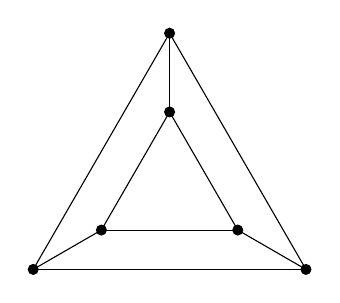
\begin{tikzpicture}
		\pgfmathsetmacro{\m}{\n-1}
		\pgfmathsetmacro{\a}{360/\n}
		\foreach \j in {0,...,\m} {
			\fill({cos(\j*\a+\b)},{sin(\j*\a+\b)})coordinate(A\j)circle(2pt);
			\fill({2*cos(\j*\a+\b)},{2*sin(\j*\a+\b)})coordinate(B\j)circle(2pt);
			\draw(A\j)--(B\j);
		}
		\foreach \j in {0,...,\m} {
			\foreach \k in {0,...,\m} {
				\ifnum\j<\k\relax
					\draw(A\j)--(A\k);
					\draw(B\j)--(B\k);
				\fi
			}
		}
	\end{tikzpicture}
	\caption{$3$-正则$(6,9)$图}
	\label{figure:图论.正则图1}
\end{figure}
\end{solution}
\end{example}

\begin{example}
%@see: 《离散数学》(邓辉文) P171 习题6.2 3.(1)
证明:\(3\)-正则图的阶数必定是偶数.
\begin{proof}
设\(G\)是\(3\)-正则\((n,m)\)图.
根据\cref{theorem:图论.握手定理} 有
\(3 n = 2 m\).
由于\(2 \mid 2 m\),
因此\(2 \mid n\),
即\(n\)必定是偶数.
\end{proof}
\end{example}

\begin{definition}
%@see: 《离散数学》(邓辉文) P170 定义6-9
在任意图\(G = (V,E)\)中,
把\[
	\Delta(G)
	\defeq
	\max_{v \in V} \deg v
\]称为\(G\)的\DefineConcept{最大度},
把\[
	\delta(G)
	\defeq
	\min_{v \in V} \deg v
\]称为\(G\)的\DefineConcept{最小度}.
\end{definition}

在\cref{figure:图论.带有自环的无向图} 中,
\(\Delta(G) = 5,
\delta(G) = 2\).

\begin{proposition}
%@see: 《离散数学》(邓辉文) P171 习题6.2 5.
设\(G\)是\((n,m)\)无向图,
则\[
	\delta(G)
	\leq
	\frac{2m}{n}
	\leq
	\Delta(G).
\]
%TODO proof
\end{proposition}

\begin{proposition}
%@see: 《离散数学》(邓辉文) P171
正则图的最大度\(\Delta(G)\)与最小度\(\delta(G)\)相等.
\end{proposition}

\begin{example}
%@see: 《离散数学》(邓辉文) P171 习题6.2 1.
证明:对于任意\(n\)阶简单图\(G\),
有\(\Delta(G) \leq n-1\).
%TODO proof
\end{example}

\begin{example}
%@see: 《离散数学》(邓辉文) P171 习题6.2 8.
设无向图\(G\)有10条边,
3度和4度顶点各2个,
其余顶点的度数均小于3.
求\(G\)至少有多少个顶点?
在最少顶点的情况下,
求\(G\)的度数序列、最大度\(\Delta(G)\)和最小度\(\delta(G)\).
%TODO \(G\)至少有7个顶点,度数序列是\(4,4,3,3,2,2,2\),最大度\(\Delta(G) = 4\),最小度\(\delta(G) = 2\)
\end{example}

\begin{definition}
%@see: 《离散数学》(邓辉文) P170 定义6-9
在有向图\(G = (V,E)\)中,
把\[
	\Delta^+(G)
	\defeq
	\max_{v \in V} \degEx v
\]称为\(G\)的\DefineConcept{最大出度},
把\[
	\delta^+(G)
	\defeq
	\min_{v \in V} \degEx v
\]称为\(G\)的\DefineConcept{最小出度},
把\[
	\Delta^-(G)
	\defeq
	\max_{v \in V} \degIn v
\]称为\(G\)的\DefineConcept{最大入度},
把\[
	\delta^-(G)
	\defeq
	\min_{v \in V} \degIn v
\]称为\(G\)的\DefineConcept{最小入度}.
\end{definition}

\begin{definition}
%@see: 《离散数学》(邓辉文) P171
对于无向图\(G = (V,E)\),
\(V = \{\AutoTuple{v}{n}\}\),
把\[
	\deg v_1,\dotsc,\deg v_n
\]
称为“\(G\)的\DefineConcept{度数序列}”.
\end{definition}

在\cref{figure:图论.带有自环的无向图} 中,
图的度数序列为\(2,5,3\).

\begin{example}
%@see: 《离散数学》(邓辉文) P171 例6-3
试讨论:是否存在一个无向图,其度数序列分别为
\(7,5,4,2,2,1\)?
\begin{solution}
由于上述度数序列中,
奇数的个数为奇数,
于是由\cref{theorem:图论.握手定理.推论} 可知,
不存在满足条件的图.
\end{solution}
\end{example}

%TODO 思考:对于给定的自然数序列\(\AutoTuple{d}{n}\),存在一个无向图(及简单无向图),其度数序列为\(\AutoTuple{d}{n}\)的充分必要条件是什么?
\begin{example}
%@see: 《离散数学》(邓辉文) P171 习题6.2 9.
证明:对于给定的自然数序列\(\AutoTuple{d}{n}\),
存在一个无向图\(G\),
其度数序列为\(\AutoTuple{d}{n}\)的充分必要条件是\[
	\sum_{i=1}^n d_i \equiv 0\pmod2.
\]
%TODO proof
\end{example}
